\chapter{Introduction}

\begin{figure}[!h]
\centering
            \subfloat[t=0]{
\includegraphics[width=.25\textwidth]{images/glider_gun/1.png}}\hfill
            \subfloat[t=10]{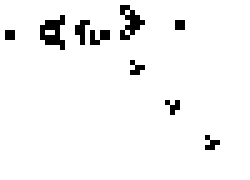
\includegraphics[width=.25\textwidth]{images/glider_gun/2.png}}\hfill
            \subfloat[t=20]{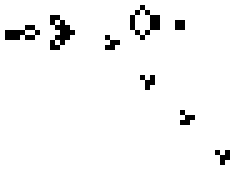
\includegraphics[width=.25\textwidth]{images/glider_gun/3.png}}\hfill
            \subfloat[t=30]{
\includegraphics[width=.25\textwidth]{images/glider_gun/1.png}}\hfill
            \caption{Gosper's Glider Gun, the first known pattern to exhibit unbounded growth in Conway's Game of Life.\cite{hickerson}}
\label{fig:gospers-glider}
\end{figure}

\section{Motivation}
Predicting effects is easier than predicting causes. This is the crux of the inverse problem in science. Estimating observations from a parameterised model of the world is easier than recovering parameters from observations. For instance, a physical model of the universe may allow us to predict the subatomic particles ejected when two protons collide at high speed but building theories \textit{based on} such collisions is difficult, especially when there are multiple equally valid explanations. Despite this, the pursuit of inverse problems is critical to advancing understanding around a system's behaviour.\\

In this thesis, we tackle an inverse problem for cellular automata (CA). We learn the parameters of CA based on observations of their state. CA are simple yet powerful models in which a discrete lattice of state-storing "cells" simultaneously perform localised computations at regular time steps. The state of each cell depends exclusively on the state of the cells in a neighbourhood around it in the previous time step. These localised interactions make CA a useful representation of physical and biological systems at all scales including fluid flow\cite{wolf2004lattice}, tumour growth\cite{deutsch2021bio, reher2017cell} and urban land use\cite{white2000high}. By automatically learning CA that accurately model such systems, we can improve our ability to predict their behaviour and develop a better understanding of their internal mechanisms. As well as simulatory models, CA are powerful computational engines owing to their inherently parallel structure. This makes learning CA a useful endeavour in the field of distributed computation as well\cite{tosic2005cellular}.\\


\section{Objectives}

Top-down investigations, which seek to classify CA and prove general results about long-term behaviour from their parameters, are vast and varied\cite{packard1985two, wolfram2002,eppstein2010growth}. In this thesis, we explore the less common bottom-up approach, where we deduce the underlying properties of a CA by observing its behaviour. Specifically, we learn the \textit{transition function} of the CA which defines how it uses its current state to generate its state in the next time step.\\

We consider three learning goals. From easiest to most difficult, they are:
\begin{enumerate}
    \item State Optimisation: Learn a CA that behaves ``similarly enough'' to the target system according to some fitness function. 
    \item State Extrapolation: Learn a CA that, for a particular initial condition, behaves exactly like the target system.
    \item Full rule dynamics: Learn a CA that, for all initial conditions, behaves exactly like the target system.
\end{enumerate}

We focus on two classes of CA in particular. The first are life-like CA which are a discrete family of models in which Conway's infamous "Game of Life" CA belongs. These CA exhibit many of the properties we wish to model in real-life systems such as chaos, nonlinear dynamics and the emergence of complexity. The second are Gray-Scott models which are continuous state CA that simulate the reactions of two diffusive chemicals. They are a discrete-time simulations of Turing's original model of morphogenesis which underlies many theories in developmental biology. For example, learning the full rule dynamics of Gray-Scott models could allow us to understand the interactions of hormones that elicit the stripes on a zebra or the spots on a leopard.\\

We use evolutionary algorithms (EAs) as our learning framework. EAs have long been held as effective tools for black-box optimisation problems. Grounded in the principles of Darwinian evolution, EAs traverse over a search space by performing selection, mutation, and crossover on a population of candidate solutions. As selection pressure grows, increasingly strong solutions emerge. Using EAs, we tackle the following objectives. Listed from easiest to most difficult, they are:

\begin{enumerate}
    \item State optimisation for life-like CA: Learn life-like CA that induce stable states with desirable properties from random initial conditions.
    \item Full rule dynamics for life-like CA: Learn the exact transition function of life-like CA based on a small sample of observations.
    \item Full rule dynamics for Gray-Scott models: Learn the exact transition function of Gray-Scott models based on a small sample of observations.
\end{enumerate}

\section{Contributions}
To achieve these objectives, this project makes the following key contributions:
\begin{itemize}
    \item \textbf{Evolutionary algorithm toolkit}\\ We build a versatile toolkit that implements evolutionary algorithms to train and optimise different classes of CA. It features support for different genotypes, loss functions, genetic operators and selection methods.
    \item \textbf{CA simulator}\\ We build simulators for discrete and continuous CA. This allows various transition functions to be implemented in the EA toolkit. These also render snapshots of the CA directly during simulation which allows animations to be automatically generated afterwards.
    \item \textbf{Procedural maze generator}\\ We write a CA-based maze generation program to test EA toolkit for state optimisation of life-like CA. The maze generator is optimised by the EA toolkit to produce ``challenging'' mazes which exhibit properties such as a long solution path and many dead ends. Mazes generated are guaranteed to have a valid solution path from start to end.
    \item \textbf{Learning life-like CA}\\ We implement a genetic algorithm that learns full rule dynamics of life-like CA. It is able to learn all 100 randomly generated test cases. On average, it searches $0.047\%$ of the search space before converging on the global optimum. This is a significant improvement over a random exhaustive search which would search $50\%$ of solutions on average.
    \item \textbf{Learning Gray-Scott CA}\\ We implement a genetic algorithm and evolutionary strategy that converge to locally optimal regions for Gray-Scott models. These regions are visualised with respect to the target in the parameter space.
    \item \textbf{Systematic analysis of life-like CA}\\ We provide an analysis of life-like CA based on repeated finite-time simulations over random initial conditions. This suggests characteristics of CA that make them easier or harder to learn automatically.
    \item \textbf{Media generation}\\ A program to convert numerical data from CA simulations into high-fidelity media. In tandem with statistical summaries, this created opportunities for qualitative analysis. This also helps provide a visual intuition for the project when communicating results.
\end{itemize}

\section{Technical Challenges}
The primary technical challenges faced during this project were:
\begin{itemize}
    \item \textbf{Building from the ground up}\\ This project is built entirely from scratch with no external libraries except simple data and image processing packages (e.g. NumPy, Pandas, Python Image Library). This involved producing implementations of cellular automata, evolutionary procedures, genetic operators, and loss functions. These components went through many iterations to ensure they were extensible and modular.
    \item \textbf{Efficient simulation}\\ Each evolutionary algorithm runs on large populations over multiple epochs. Fitness is calculated by repeated simulation of individual CA which means that thousands of simulations need to be run for each experiment. Therefore, the simulator must be efficient. This is especially important for the Gray-Scott simulator which uses numerical integration to approximate solutions for 2D partial differential equations. Producing a realistic yet efficient simulation in this case required much experimentation.
    \item \textbf{Avoiding local optima}\\ Evolutionary algorithms are very susceptible to premature convergence to local optima. It is infeasible to test every combination of evolutionary techniques, genetic operators, loss functions, and hyperparameters. Therefore, the design of these algorithms had to be approached with forethought to maximise the chances of avoiding local optima. 
    \item \textbf{Efficient experimentation}\\ Hyperparameter tuning and evaluation of each technique required running large-scale experiments. With the computational resources available, it was important to consider which experiments would provide the most insight relative to the time taken to run them. As an example, simulation of all life-like CA rules for exploratory analysis required 25 hours on a 4-core, 8GB AMD-Compute cluster.
\end{itemize}

\section{Ethical Considerations}
Technologies falling in the broad field of self-organising systems, distributed systems, and automated systems can be misused. This presents some ethical issues that are worth discussing.\\

One area of legal concern is the infringement of copyright law when selecting training data. To train cellular automata for real world applications, we would use many datasets collected from physical, biological, or chemical experiments. As a collection of facts, such data is usually exempt from copyright law. However, training data can, in theory, be derived work which puts it in the remit of copyright law. Examples include certain terrain maps or urban land use reports. When choosing point data to train on, we will ensure that they do not fall under copyright restrictions and that they are legally suitable for academic use.\\

An area of societal concern is the explainability of CA systems. Suppose a CA model is built to forecast the spread of an epidemic and results are used to guide public policy. While this kind of problem is particularly pertinent to black-box systems like artificial neural networks, it is less of a concern for CA which tend to be simplistic and more transparent. This work does not delve into CA models with any public or business use.\\

An area of ethical concern is the general application of cellular automata in distributed technology like swarm robotics. Such systems can have military applications. It could be argued that this research could pave the way for highly distributed swarms of drones or ground robots that are capable of complex self-organising behaviour. However, this is unlikely to be a true concern since we only discuss theoretical concepts in this paper with little discussion about physical applications in robotics. Furthermore, this research is only in its very preliminary stages. As a relatively mathematical project, there are few major ethical factors to consider here.\\